\section{Methodology}\label{sec:methods}

As described above, the main contribution of Tran and Yates in the discussed work is to consider entities independently of the underlying large language model. In order to do so, they combine embeddings of an arbitrary large language model with embeddings of the entities from the respective documents and queries. For the embeddings of entities, they introduce some kind of multiple views on entities: Different sets of entities within queries and documents represent different perspectives on the queries and documents. Depending which view a query displays, different documents or parts of documents might be relevant.

In contrast to the previously described methods in \autoref{subsec:dense}, the separate embeddings of queries and documents are not inserted as components into a learned framework, but are merely merged into a joint vector space. As a result, a final embedding in the joint vector space is derived, which is used to calculate similarities between different vectors. Therefore, Tran and Yates, stick to the bi-encoder model (see \autoref{sec:introduction}), which allows indexing of embeddings for documents and enables fast ranking computations via ANN search. 

\subsection{General Model}\label{subsec:general_model}

The proposed method of Tran and Yates incorporates embeddings of documents and entities independently. To achieve a joined vector space, they merge embeddings of both for each query and document. This general approach is illustrated in \autoref{fig:general_model}: Since Tran and Yates follow the bi-encoder approach (see \autoref{sec:introduction}), embeddings for queries and documents are created independently of each other using a pre-trained large language model. 

\begin{figure}[!htb]
    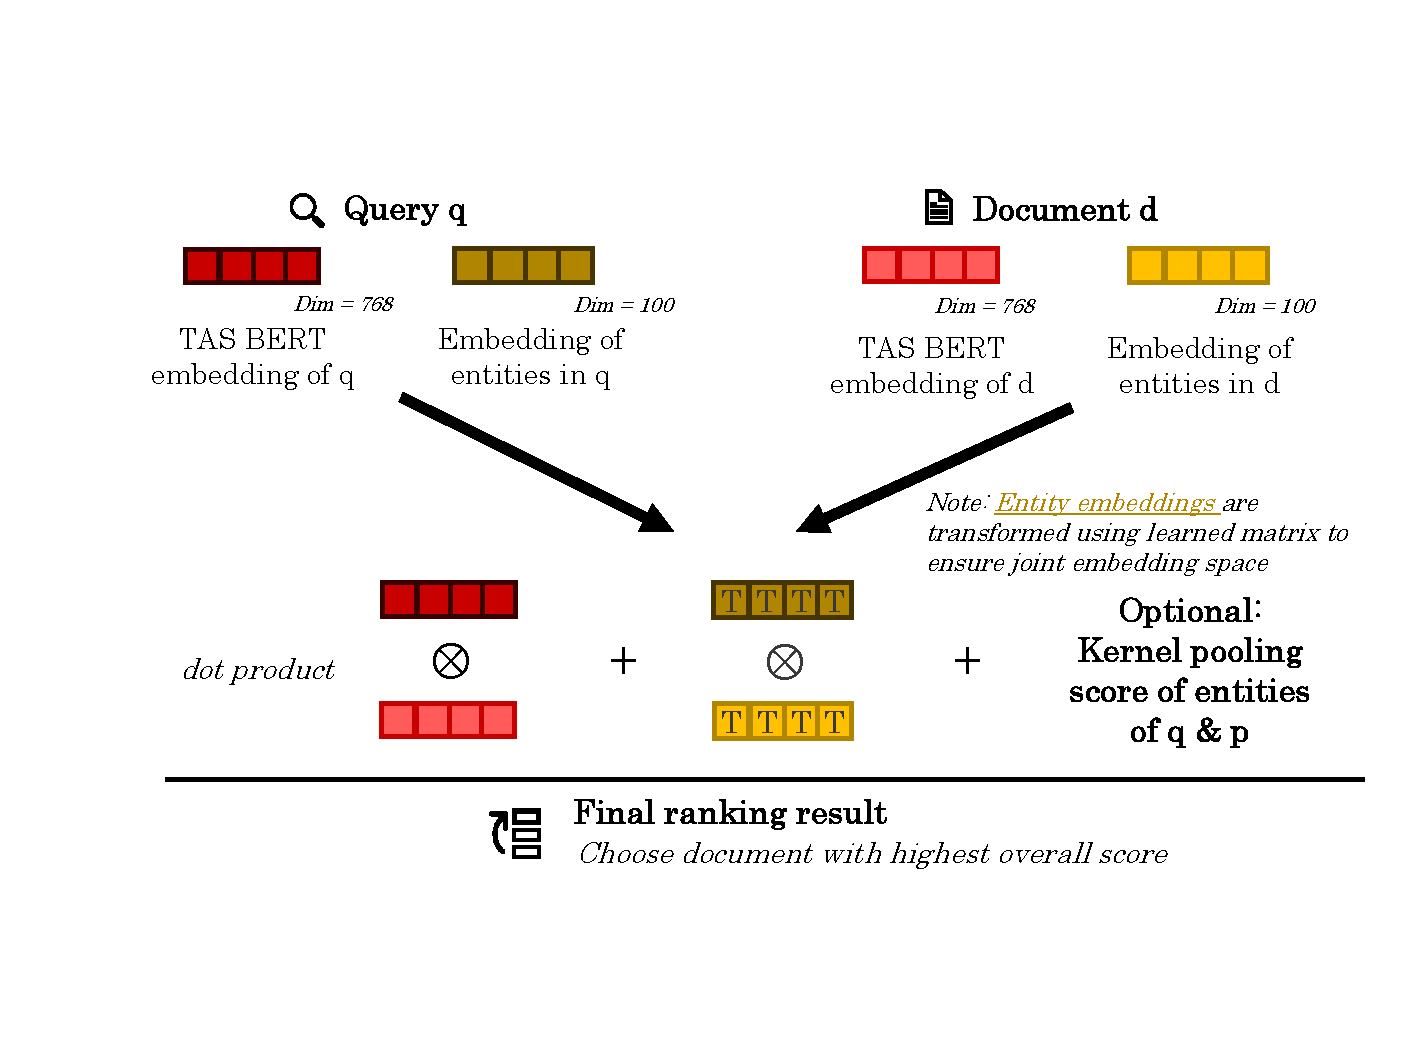
\includegraphics[trim={1.5cm 3cm 1.5cm 3cm}, clip, width=\textwidth]{resources/general_model} 
    \caption{General model}
    \label{fig:general_model}
\end{figure}

In their work, Tran and Yates use a distilled version of BERT (Sanh et al. \cite{sanh2019distilbert}), which was fine-tuned via TAS BERT approach by Hofst{\"a}tter et al. \cite{tasbert} for information retrieval task. The distilled version of BERT is used by Tran and Yates with the objective of maintaining low computational costs while losing little effectiveness. 

The term TAS BERT of the method of Hofst{\"a}tter et al. refers to the term 'topic aware sampled BERT', whereby sampling during training process of the information retrieval system is meant. In concrete, within TAS BERT approach the queries of the training dataset are clustered in advance based on different topics. During training process, query samples are extracted only from clusters of identical topics. This is intended to make the information retrieval model more sensitive to differing topics. 

In a usual dense retrieval setting, the generated embeddings of tokens are then compared using similarity measurements. When a query is submitted to a system, the ranking of the best documents with respect to the query is carried out, based on the calculated similarity score between the duets of the given query and all documents. 

For their model, Tran and Yates use the identical principle, but enhance it with embeddings of entities. In addition to the textual embeddings of a pre-trained language model, for each query and each document a single entity embedding is generated. Subsequently, the textual embedding is combined with the entity embedding in order to create an embedding that contains both the information about the semantic context and the information about the entities. The term combination here refers to concatenation of both vectors. 

Experimental results of Tran and Yates showed that concatenation yields the best results for combining both embeddings of text and entities compared to others like max pooling and sum pooling. \autoref{tab:operator} displays the respective analysis of Tran and Yates based on their experimental setup, which is introduced in detail in \autoref{sec:results}. Apart from the analytical point of view, the approach of concatenation offers the advantage that it can be understood quite intuitively.

\begin{table}[!htb]
    \centering
    \begin{tabular}{llll}
    \hline
    \multirow{2}{*}{\textbf{Operators}} & \multicolumn{3}{c}{\textbf{MS MARCO Dev}}   \\
                                      & \textbf{nDCG} & \textbf{MRR} & \textbf{MAP} \\
    \hline
    Sum & 0.393 & 0.335 & 0.339 \\
    Max & 0.388 & 0.330 & 0.334 \\
    Concat & 0.396 & 0.341 & 0.343 \\
    \hline
    \end{tabular}
    \caption{Varying Aggregation Operators of Embedding Concatenation}
    \label{tab:operator}
\end{table}

However, there is an issue to be solved in the context of concatenation: Since the vectors of the word embeddings and the entity embeddings are generated in a different vector space, this setup leads to biased similarity results. More precisely, the dimension of the word embeddings of the distilled TAS BERT model is 768 and of the word embeddings 100. Moreover, the magnitudes of the embeddings do not necessarily coincide. To overcome this problem, Tran and Yates introduce a transformation matrix $W \in \mathbb{R}^{100 \times 100}$ for the vectors of the embeddings. So let $\mathbf{E}(t)$ be the embedding of entities of text $t$, the transformed entity embedding is given as:
\begin{align}
    \mathbf{R}_{entity}(t) = W^T \cdot \mathbf{E}(t)
\end{align}
The values of the matrix are determined during the training process of the entire model and thus reflect a meaningful transformation of the embeddings into a joint vector space. 

Given text $t$ and its corresponding word embedding $\mathbf{R}_{text}(t)$ derived by the pre-trained language model, the final vector representation of $t$ is then calculated as:
\begin{align}
    \mathbf{R}_{final}(t) &= \mathbf{R}_{text}(t) \oplus \mathbf{R}_{entity}(t)
\end{align}

As a further optional addition to their model, Tran and Yates include an external scoring source that measures the relationship between query entities and documents. They use a kernel pooling score that is intended to measure the importance of entities of queries which also occur within documents. Accordingly, this approach requires knowledge of the query and document at runtime. Therefore, this approach belongs to methods interaction-based approaches of incorporating entities within retrieval tasks, as described in \autoref{sec:related_work}.

This kernel pooling score, called KNRM-signal will be elaborated in detail in the following subsection. Together with the KNRM-signal $S_{knrm}$ of a query $q$ and a document $d$ the final vector representation of the model of Tran and Yates resolves to 
\begin{align}
    \mathbf{R}_{final\_knrm}(t) =
    \begin{cases}
         \mathbf{R}_{text}(t) \oplus \mathbf{R}_{entity}(t) + 1 & t \text{~is query} \\
         \mathbf{R}_{text}(t) \oplus \mathbf{R}_{entity}(t) + S_{knrm}(t) & t \text{~is document} \label{eq:knrm}
    \end{cases}
\end{align}

Since the interaction of entities in queries with each other is always ideal, the maximum value $S_{knrm}(t)$ will be reached whenever $t$ is a query. As shown in \autoref{subsec:knrm}, the supremum of $S_{knrm}(t)$ is 1, therefore the value for $S_{knrm}(t)$ is set to 1, if t is a query.

\subsection{KNRM Signal}\label{subsec:knrm}

Tran and Yates introduce the KNRM signal, originally developed by Xiong et al. \cite{xiong2017end}, as an additional scoring mechanism to extend their basic approach by a separate framework. Unlike its original use, Tran and Yates adapt the KNRM model to specifically capture the interaction between entities in queries and documents. The calculation of the KNRM signal follows these steps:

\begin{enumerate}
    \item Let $X(q)$ be the set of all entity embeddings within query $q$, $X(d)$ any set of entity embeddings which occur in document $d$. For EVA Single and EVA Single-QA models (see \autoref{subsec:models}) $X(d)$ contains all entities with the given document, for EVA Multi (see \autoref{subsec:models}) $X(d)$ contains only entities of specific subsets of entities of $d$. The entity interaction matrix is defined as: 
    \[T_{i,j} := sim(X_i(q), X_j(d)) \text{~,}\]
    where $X_i(q)$ and $X_j(d)$ are the $i$-th and $j$-th embedding of $q$ and $d$. The similarity function is given as cosine similarity. Embeddings are generated via Wikipedia2Vec (Yamada et. al \cite{yamada2018wikipedia2vec}), as described in \autoref{subsubsec:extracting_entities}.
    \item Build k kernels using radial basis function, which creates differentiable histograms around given $\mu$ and $\sigma^2$.
    \[ K_l(X_i(q)) = \sum_{j=1}^{|X(p)|}\exp\left(-\frac{(T_{i,j}-\mu_i)^2}{2\sigma_i^2}\right)\]
    \item Pool / Summarize the k results into a k-dimensional feature vector: \[\overrightarrow{K(X_i(q))} = [K_1(X_i(q)), \ldots, K_k(X_i(q))]\]
    \item Build kernel-pooled representation $\phi(T)$ by calculating log-sum for each query entity: \[\phi(T) = \sum_{i=1}^{|X(q)|} \log \overrightarrow{K(X_i(q))}\]
    \item Get final kernel pooling score by applying a learned ranking layer. Note that $\tanh(\cdot) \in (-1, 1)$ and therefore $\sup S_{knrm} = 1$: \[ S_{\text{knrm}} = \tanh(w^T\phi(T) + b) \]
  \end{enumerate}

Despite being an interaction-based model that requires scoring during runtime for all query-document pairs, the computational complexity of the KNRM approach remains limited. The computations involved are relatively straightforward, and the additional learned layer does not significantly increase the computational overhead. Furthermore, these computations can be performed in parallel with the other components of Tran and Yates' approach. Empirical results concerning the latency of the models, with and without the KNRM signal, validate this assertion (see \autoref{sec:results}).

\subsection{Generating Entity Embeddings\label{subsec:entity_embeddings}}

As described in \autoref{subsec:general_model}, Tran and Yates create embeddings for both word tokens and entities in queries and documents. While the word token embeddings are generated using TAS BERT through the dense retrieval approach, the primary focus of their contribution lies in the creation of entity embeddings. In particular, since queries and documents usually contain more than one entity, they need to be aggregated to a single embedding.

In order to do so, the example given in \autoref{fig:example} shall be introduced: Given the query 'Favourite book bert sesame street' and a corresponding document that mentions Bert as a character of Sesame Street who enjoys the book Boring Stories, there are three entities: Bert, Sesame Street, and Boring Stories.

\begin{figure}[!htb]
    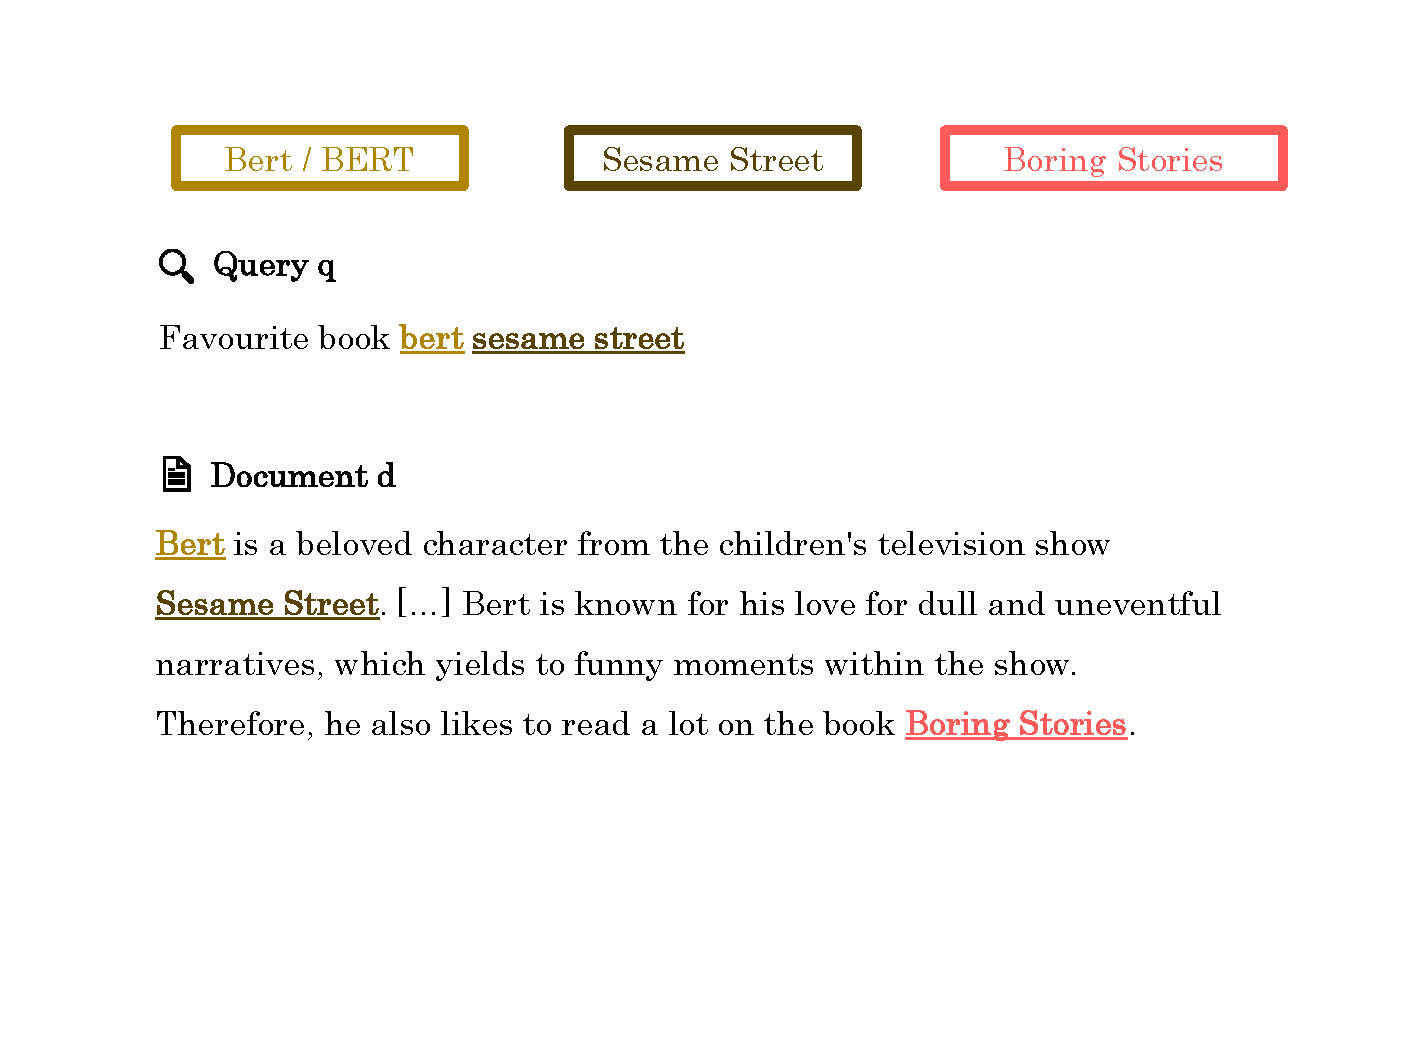
\includegraphics[trim={1.5cm 5.5cm 1.5cm 2cm}, clip, width=\textwidth]{resources/example} 
    \caption{Example query and example document}
    \label{fig:example}
\end{figure}

\subsubsection{Extracting Entities}\label{subsubsec:extracting_entities}

To aggregate multiple entities in a document or query, Tran and Yates first extract these entities from the text using external frameworks Dexter (Ceccarelli et al. \cite{ceccarelli2013dexter}) and Wikipedia2Vec (Yamada et. al \cite{yamada2018wikipedia2vec}).

The Dexter framework is an entity linkage system that resolves entity mentions in text to corresponding entities in a knowledge base. In particular, Dexter employs a combination of methods, including named entity recognition and pattern matching, to perform this task. 

Wikipedia2Vec, on the other hand, leverages the structure of Wikipedia to generate dense vector representations (embeddings) for words, articles, and entities. It utilizes the Word2Vec algorithm (Mikolov et al. \cite{mikolov2013distributed}) to capture semantic relationships from Wikipedia, producing high-dimensional embeddings.

The extraction procedure involves submitting a document or query to Dexter, which extracts entity mentions from the given text. These entity names are then passed on to the knowledge base, which transforms them into embeddings. Wikipedia2Vec provides vectors in dimension 100 as default, Tran and Yates keep this value in their model. \autoref{fig:entity_extraction} visualizes this process.

\begin{figure}[!htb]
    \centering
    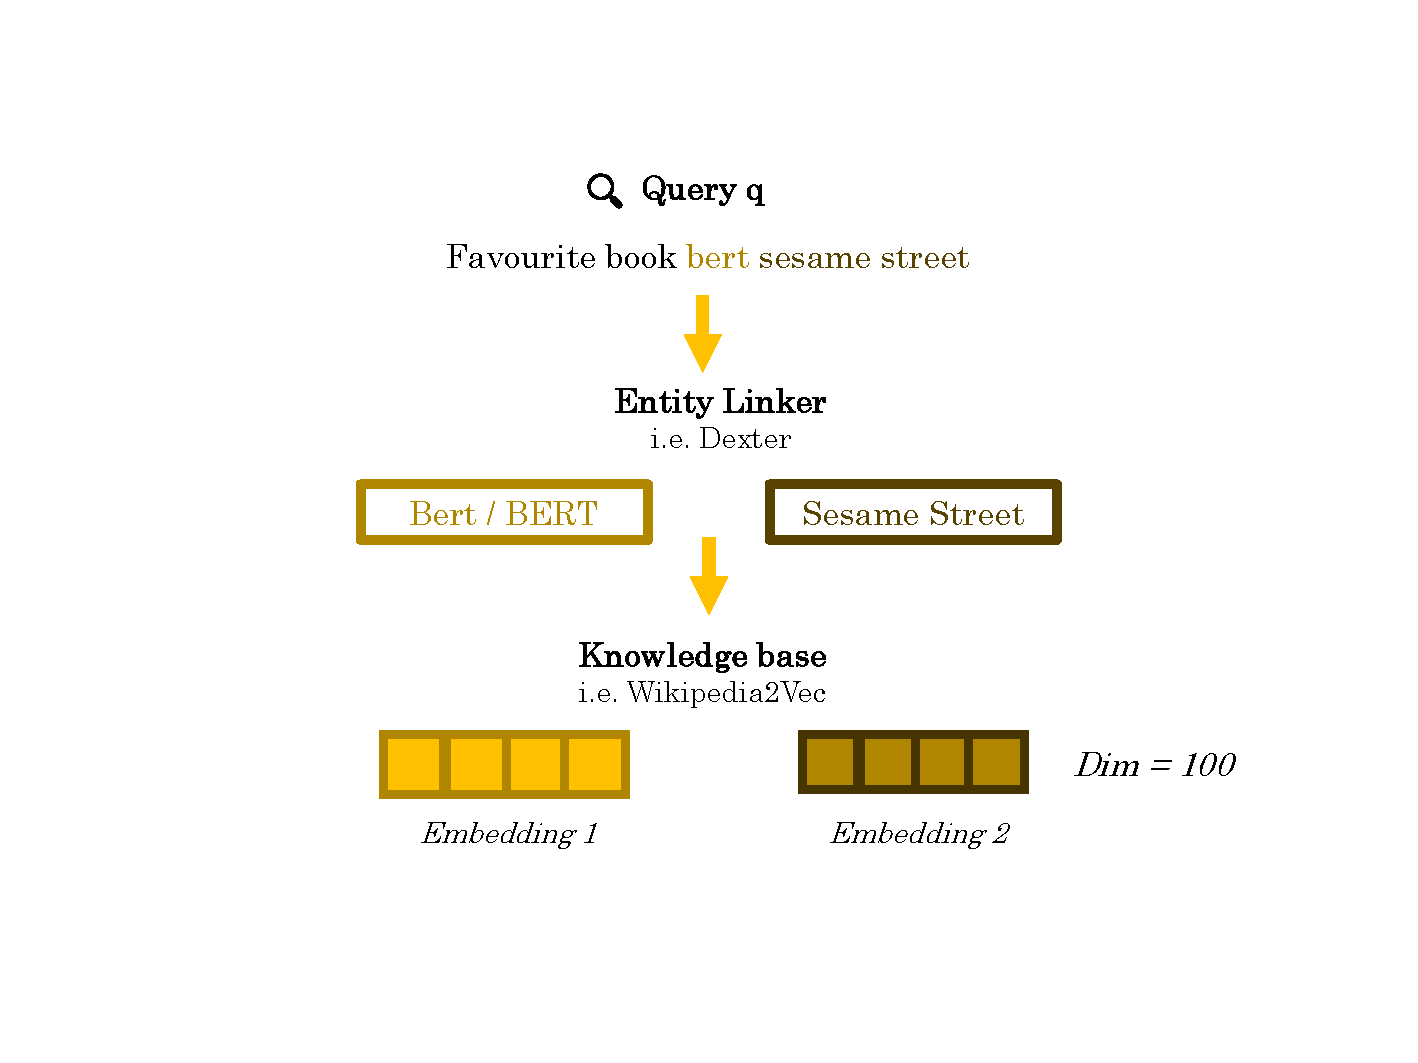
\includegraphics[trim={2cm 3cm 2cm 2cm}, clip, width=0.9\textwidth]{resources/entity_extraction} 
    \caption{Process of entity extraction}
    \label{fig:entity_extraction}
\end{figure}

\subsubsection{Combining Entities for Queries}\label{subsub:generating_queries}

For now, multiple embeddings for each entity within a query or a document are generated by applying the procedure outlined in \autoref{subsubsec:extracting_entities}. The aggregation of these generated embeddings differs based on whether a query or a document is considered, given the usual brevity of queries compared to documents.

For queries, Tran and Yates adopt a straightforward approach. They aggregate the embeddings of entities by averaging all entity embeddings across all dimensions. \autoref{fig:queries} visualizes this procedure.

\begin{figure}[!htb]
    \centering
    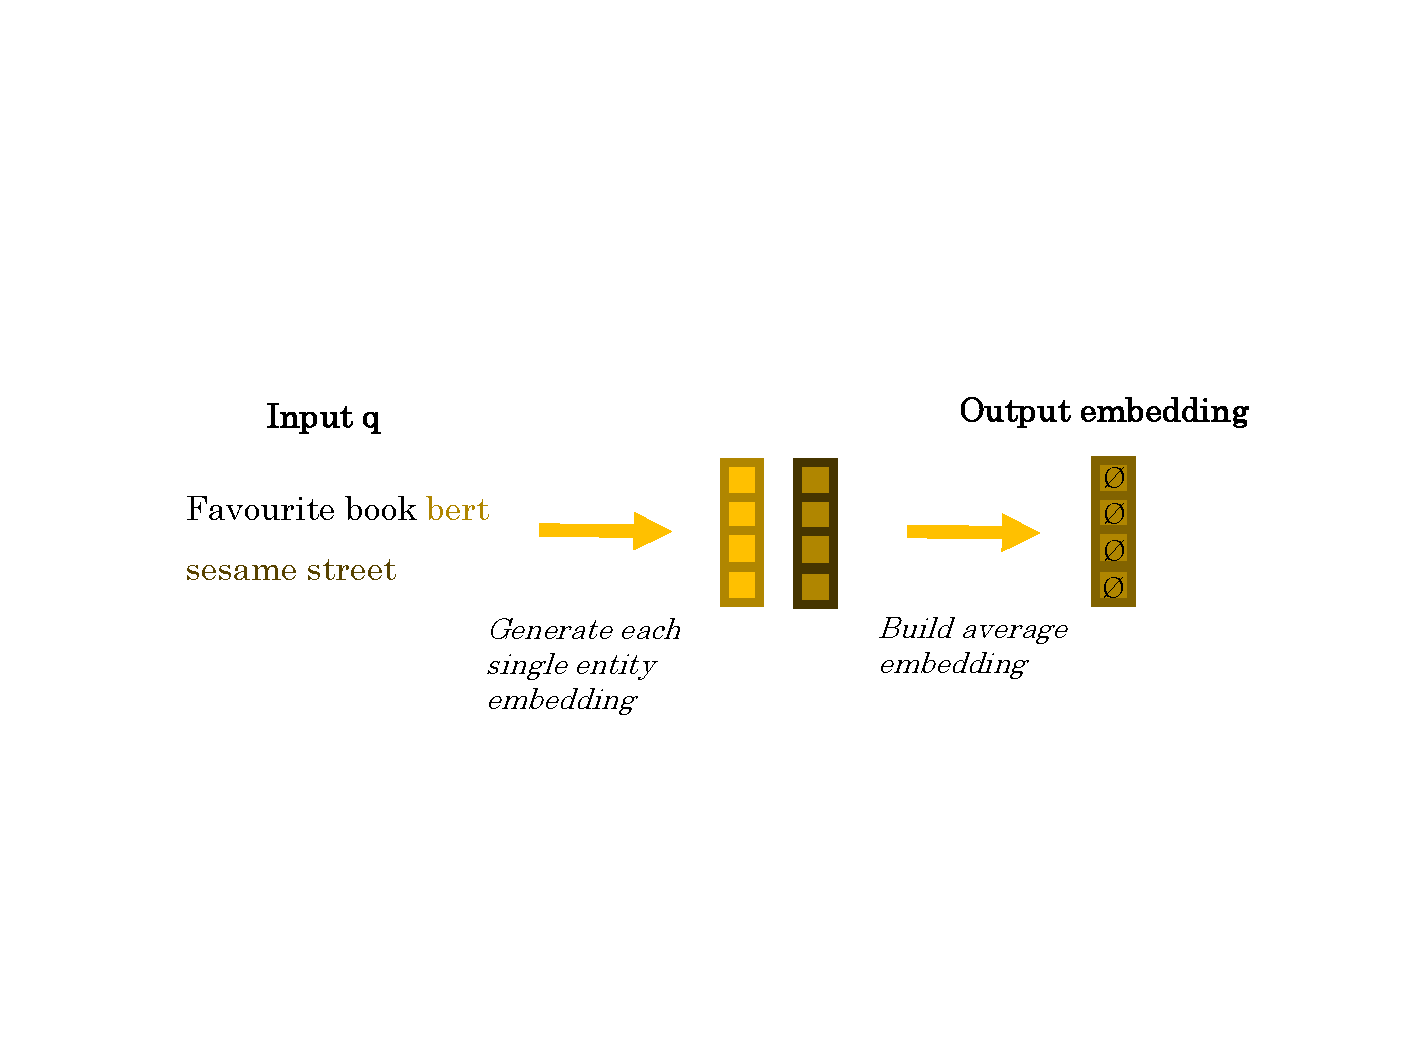
\includegraphics[trim={2cm 6cm 2cm 6cm}, clip, width=\textwidth]{resources/queries} 
    \caption{Process of generating a single entity embedding for a query}
    \label{fig:queries}
\end{figure}

\subsubsection{Combining Entities for Documents}\label{subsec:models}

Documents usually contain many different entities, as the example in \autoref{fig:example} indicates. Additionally, documents might also cover different aspects of a topic, so entities from very different areas might appear within them. This factor adds more complexity to the aggregation of embeddings for documents than for queries. To overcome this issue, Tran and Yates elaborated three different methods to aggregate embeddings of documents, which build upon each other:

\begin{itemize}
    \item Single Entity Representation (EVA Single)
    \item Query-Aware Single Entity Representation (EVA Single-QA)
    \item Multiple Entity View Representation (EVA Multi)
  \end{itemize}

The term EVA refers to \underline{E}ntity \underline{V}iews in Dense Retriev\underline{a}l. The concept of Entity Views, the name-giving term for the paper by Tran and Yates, is used in particular in the third method EVA Multi and will be introduced in the following.

\paragraph*{EVA Single}

The first approach of aggregating the entities of a document is similar to the one used for queries. The idea of the Single Entity Representation approach is to extract all entities of a document and then create a single average output embedding. Analogous to \autoref{fig:queries} for queries, this approach is visualized in \autoref{fig:eva_single}.

\begin{figure}[!htb]
    \centering
    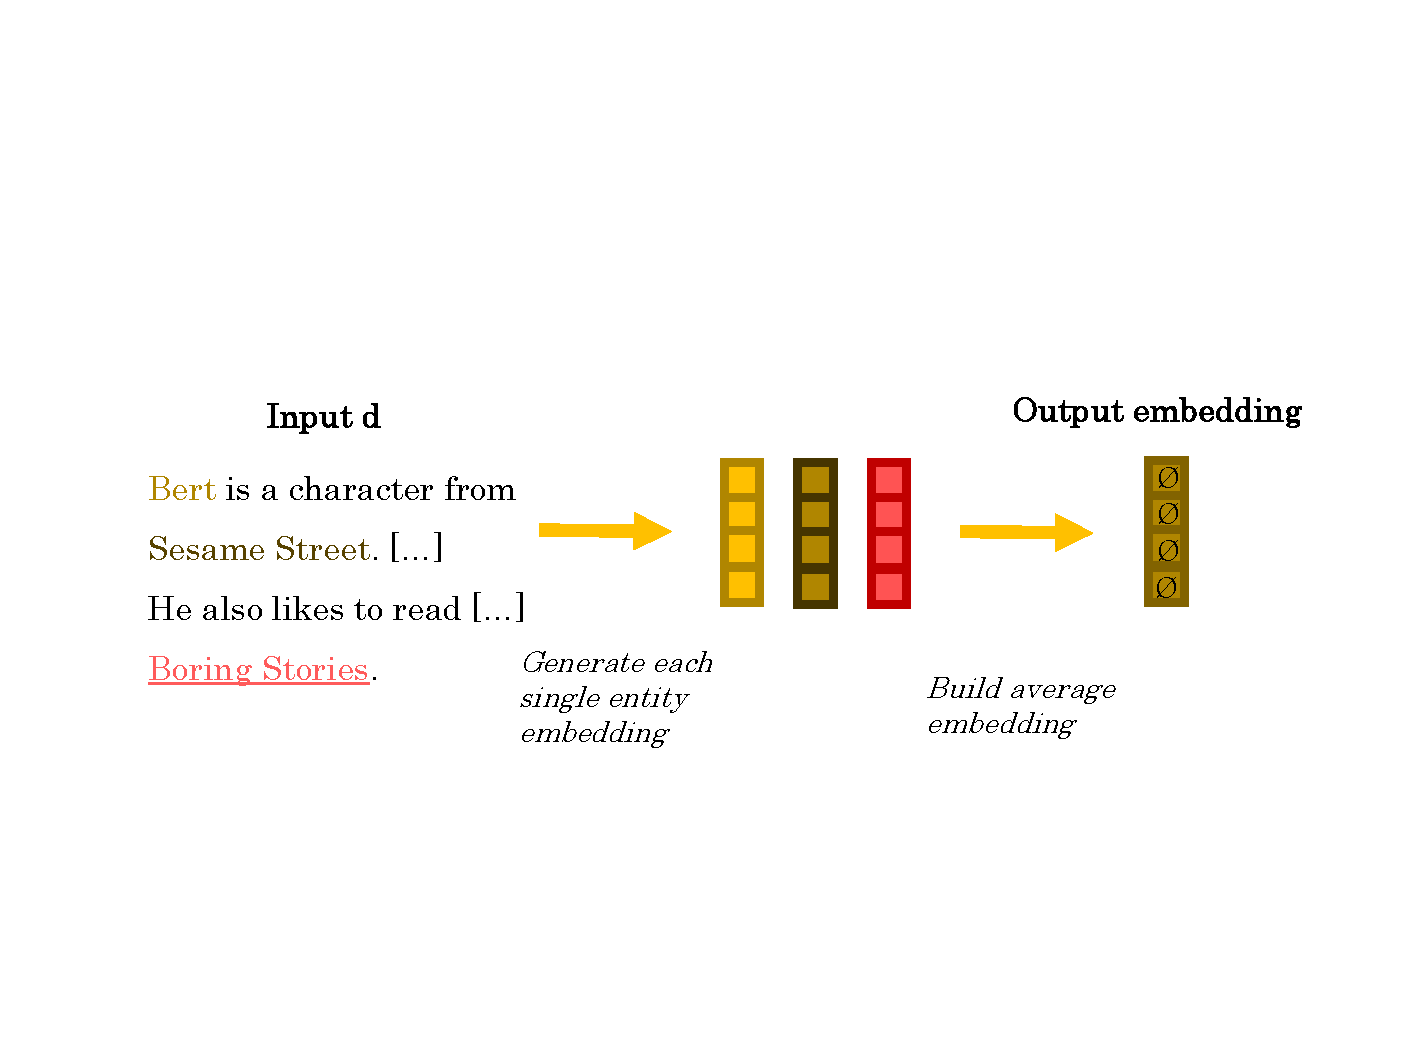
\includegraphics[trim={2cm 6cm 1.5cm 6cm}, clip, width=\textwidth]{resources/eva_single} 
    \caption{Process of generating an entity embedding for a document following the EVA Single approach}
    \label{fig:eva_single}
\end{figure}

This approach does not take into account that documents can cover various topics. The query information is completely discarded and thus partially irrelevant entities are accounted for calculations of the output embedding. This leads to a bias within the ranking results, as it can be observed in \autoref{sec:results}.

\paragraph*{EVA Single-QA}

To address this problem, Tran and Yates introduce the Query-Aware Single Entity Representation, which creates embeddings focusing on the needs of the query. However, this requires the assumption that the query is known before calculations, which leads to increased computational complexity. This is due to the fact that computations for all duets of query and documents must now be performed during runtime, precomputations of embeddings for documents and indexing is no longer possible. This effect is reflected within the results (see \autoref{sec:results}), which prove a high latency in the case of the EVA-Single QA approach.

The underlying idea of the EVA single QA model is to filter the entities of a document based on the information of a given query and select only entities with high similarity to a query entity. \autoref{fig:eva_single_qa} visualizes this process.

\begin{figure}[!htb]
    \centering
    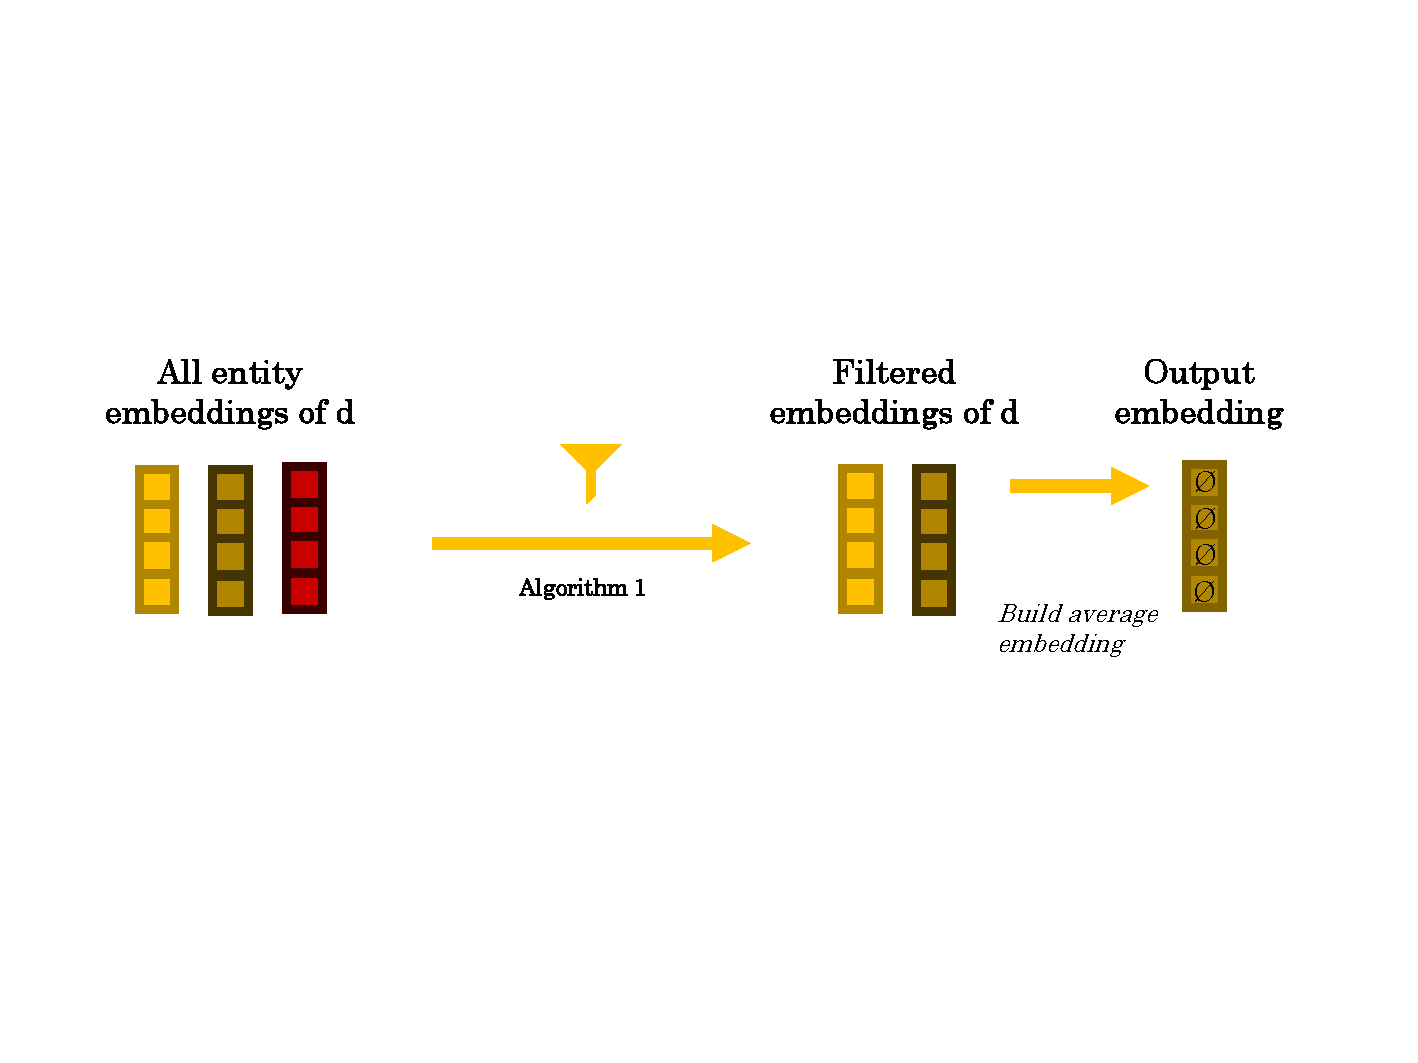
\includegraphics[trim={1cm 6.5cm 2cm 6cm}, clip, width=\textwidth]{resources/eva_single_qa} 
    \caption{Process of generating an entity embedding for a document following the EVA Single-QA approach}
    \label{fig:eva_single_qa}
\end{figure}

Filtering is done using algorithm \ref{alg:query-aware-entity-representation}, which is applied to all duets of a query $q$ and document $d$: For each entity within $q$ the algorithm searches for the entity within $d$ having the maximum cosine similarity. If this similarity extends some threshold, the respective entity of $d$ will be added to the filtered list $X_{focus}(d)$. As a final step, the single output embedding for document $d$ is calculated as the average of all entity embeddings within the filtered list $X_{focus}(d)$.

\begin{algorithm}[!htb]
    \caption{Query-aware document entity representation}
    \label{alg:query-aware-entity-representation}
    \begin{algorithmic}[1]
    \REQUIRE Query $q$ and document $d$, threshold $\alpha$
    \ENSURE Filtered entity embedding list $X_{focus}(d)$ of $d$
    
    \STATE $X(q) \leftarrow$ set of embeddings of entities in $q$
    \STATE $X_{focus}(d) \leftarrow \{\}$
    \FOR{$e$ in $X(q)$}
        \STATE $e^* \leftarrow$ entity embedding in $d$ having the maximum cosine similarity with $e$
        \IF{cosine similarity$(e^*, e) > \alpha$}
            \STATE $X_{focus}(d) \leftarrow X_{focus}(d) \cup \{e^*\}$
        \ENDIF
    \ENDFOR
    \RETURN $X_{focus}(d)$
    \end{algorithmic}
\end{algorithm}

\paragraph*{EVA Multi}

The EVA single-QA approach suffers from the issue that queries must be known before algorithm \ref{alg:query-aware-entity-representation} can be applied and the query-aware document representation can be retrieved. With the third approach, called EVA-Multi, Tran and Yates have found a solution to this problem with only minor negative side effects.

They analyzed their training data and realized that the number of entities in queries do not exceed two in the vast majority of instances. Based on the experimental setup described in \autoref{sec:results}, they found that 99.6 \% of the 300,000 training instances and 99.5 \% of test instances in the MS Marco Dev dataset contain two or fewer entities. \autoref{tab:query_statistics} shows the respective analysis of queries. Therefore, Tran and Yates focused their research on the assumption that it is sufficient to consider a maximum of two entities in queries.

\begin{table}[!htb]
    \centering
    \small
    \begin{tabular}{lp{2cm}cp{2cm}c}
    \hline
    \multirow{2}{*}{\textbf{Entities}} & \multicolumn{2}{c}{\textbf{Training Queries}} & \multicolumn{2}{c}{\textbf{Testing Queries}} \\
                                 & \textbf{Count}           & \textbf{Fraction}          & \textbf{Count}           & \textbf{Fraction}          \\
    \hline
    0 & 130,353 & 0.435 & 3,442 & 0.483 \\
    1 & 149,073 & 0.497 & 3,232 & 0.454 \\
    2 & 19,207 & 0.064 & 416 & 0.058 \\
    3+ & 1,367 & 0.004 & 37 & 0.005 \\
    \hline
    \textbf{Total} & 300,000 &  & 7,127 &  \\
    \textbf{Average} & 0.640 &  & 0.587 &  \\
    \hline
    \end{tabular}
    \caption{Summary statistics of the queries.}
    \label{tab:query_statistics}
\end{table}

If one applies algorithm \ref{alg:query-aware-entity-representation} under this assumption, one notices that at most two entities remain in the filtered embedding list $X_{focus}$. This is due to the fact that the algorithm iterates over the set of all entities in the given query once. Since $X_{focus}$ therefore only contains no item, a single item or at maximum two items, the amount of all possible sets that are eligible for $X_{focus}$ is limited by $|\{\}| + |X(d)| + \binom{|X(d)|}{2}$, where $|X(d)|$ corresponds to the number of entities in $d$. 

Tran and Yates take advantage of this and introduce clusters of entities that can be seen as different views on a document. For the EVA Multi approach, all possible single itemsets and sets of pairs of the entities are generated. Sets of pairs are only considered, if cosine similarity between the two items within a pair extend a predefined threshold $\beta$ to ensure only reasonable entity views are generated. Final output embeddings are again calculated by averaging the embeddings of all items within each set. When applying the optional KNRM signal (see \autoref{subsec:knrm}) to this approach, the entity interaction matrix $T$ is build only upon the set of the entity embeddings of a single cluster and not on all entities within the respective document.

\begin{figure}[!htb]
    \centering
    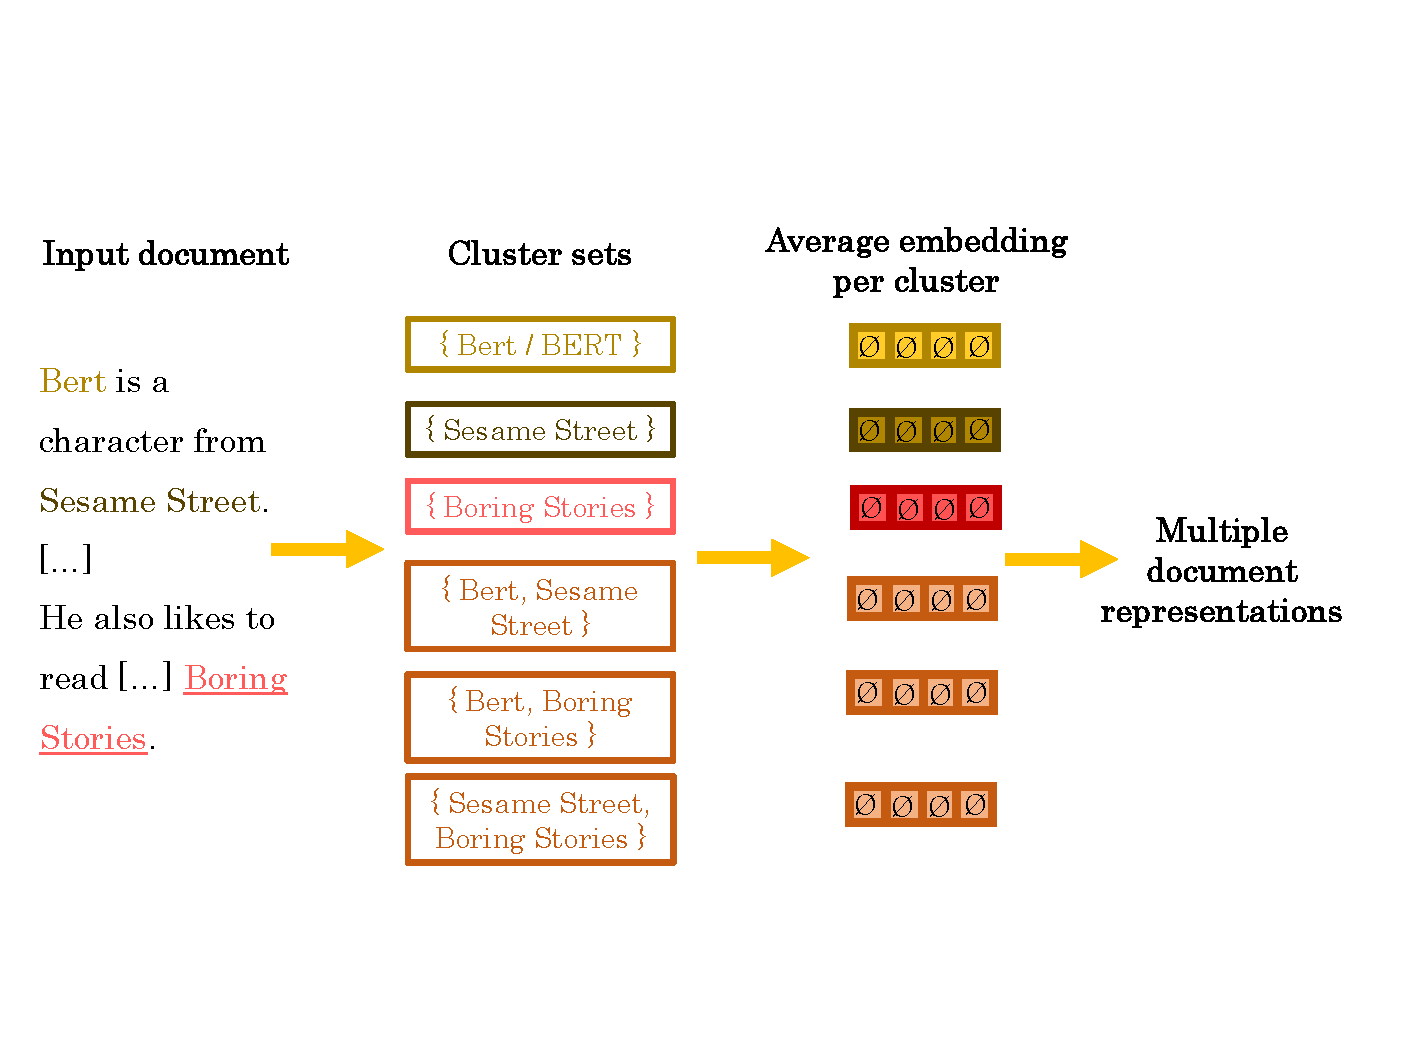
\includegraphics[trim={0cm 3cm 0cm 3.5cm}, clip, width=\textwidth]{resources/eva_multi} 
    \caption{Process of generating entity embeddings for a document following the EVA Multi approach}
    \label{fig:eva_multi}
\end{figure}

All the calculations can be performed independently of the information about queries and thus allow indexing. In contrast to the two previously mentioned methods EVA Single and EVA Single-QA, several entity output embeddings are now generated per document, which have to be taken into account during retrieval ranking. 

\autoref{fig:eva_multi} visualizes the process of generating the embeddings of multiple entity views / clusters. For the given example of three entities within an input document, six different views on entities and document entity representations are generated.


